\documentclass[tikz]{standalone}
\begin{document}

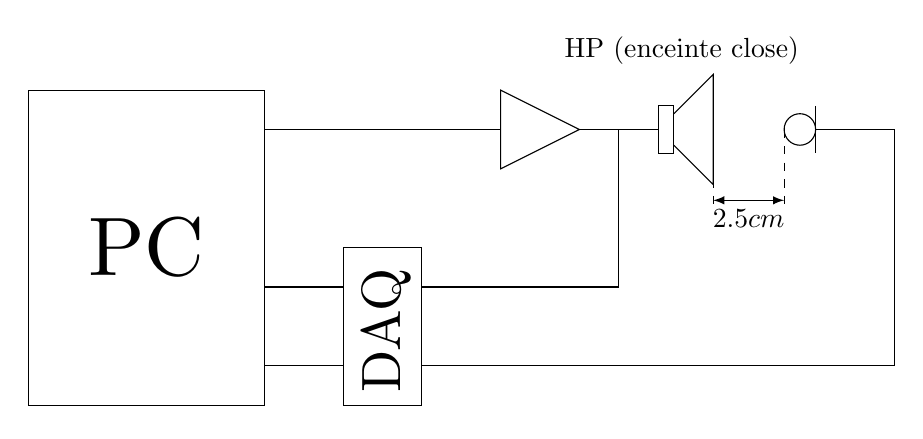
\begin{tikzpicture}

    % pc
    \draw (0,0) rectangle (3,4);

    % ampli
    \draw (3,3.5) -- (6,3.5);
    \draw (6,4) -- (7,3.5) -- (6,3) -- cycle;

    % carte acqui
    \draw (3,0.5) -- (4,0.5);
    \draw (3,1.5) -- (4,1.5);
    \draw (4,0) rectangle (5,2);

    % HP
    \draw (8,3.2) rectangle (8.2,3.8);
    \draw (8.2,3.7) -- (8.7,4.2) -- (8.7,2.8) -- (8.2,3.3);

    % micro
    \draw (9.8, 3.5) circle (.2);
    \draw (10,3.8) -- (10,3.2);

    % acqui -> amp
    \draw (5,1.5) -- (7.5,1.5) -- (7.5,3.5);
    % amp -> HP
    \draw (7,3.5) -- (8,3.5);
    % mic -> acqui
    \draw (10,3.5) -- (11,3.5) -- (11,0.5) -- (5,0.5);

    % texts
    \draw (4.55,0.95) node[rotate=90, scale=2] {DAQ};
    \draw (1.5,2) node[scale=3] {PC};
    \draw (8.3,4.2) node[above] {HP (enceinte close)};

    % distance HP -> mic
    \draw[dashed] (9.6,3.5) -- (9.6,2.5);
    \draw[dashed] (8.7,3.5) -- (8.7,2.5);
    \draw[<->, >=latex] (8.7,2.6) -- (9.6,2.6) node[midway,below] {$2.5cm$};


\end{tikzpicture}

\end{document}
